\documentclass[11pt]{amsart}
\usepackage[hmargin=1.2in,vmargin=1.05in]{geometry}
\usepackage{amsmath,amssymb,amsthm}
\usepackage{graphicx}
\usepackage{booktabs}
\usepackage{microtype}
\usepackage{tikz}
\usetikzlibrary{arrows.meta}
% Shared project math macros. Edit in Manuscripts → Project macros.
\newcommand{\im}{\text{im}}
\newcommand{\sgn}{\text{sgn}}
\newcommand{\eps}{\epsilon}
\newcommand{\Hom}{\text{Hom}}

\newcommand{\F}{\mathbb{F}}
\newcommand{\N}{\mathbb{N}}
\newcommand{\Z}{\mathbb{Z}}
\newcommand{\Q}{\mathbb{Q}}
\newcommand{\Qbar}{\overline{\mathbb{Q}}}
\newcommand{\R}{\mathbb{R}}
\newcommand{\C}{\mathbb{C}}
\newcommand{\G}{\mathbb{G}}
\newcommand{\A}{\mathbb{A}}
\newcommand{\bbA}{\mathbb{A}}
\newcommand{\bbH}{\mathbb{H}}
\newcommand{\bbP}{\mathbb{P}}
\newcommand{\bbS}{\mathbb{S}}
\newcommand{\bbX}{\mathbb{X}}
\newcommand{\Oh}{\mathscr{O}}
\newcommand{\Prime}{\mathscr{P}}
\newcommand{\Tree}{\mathsf{T}}
\newcommand{\T}{T_{(2)}}
\newcommand{\Gr}{\text{Gr}}
\newcommand{\Gal}{\mathsf{Gal}}

\newcommand{\GL}{\mathsf{GL}}
\newcommand{\PGL}{\mathsf{PGL}}
\newcommand{\SL}{\mathsf{SL}}
\newcommand{\SO}{\mathsf{SO}}
\newcommand{\PSL}{\mathsf{PSL}}
\newcommand{\Isom}{\mathsf{Isom}}
\newcommand{\tr}{\mathsf{tr}}
\newcommand{\mat}[4]{\begin{pmatrix} #1 & #2 \\ #3 & #4\end{pmatrix}}

% For the ping-pong demo
\newcommand{\abs}[1]{\left|#1\right|}
\newcommand{\gen}[1]{\langle #1 \rangle}
\newcommand{\RP}{\mathbb{RP}}

\graphicspath{{figures/}}
\setlength{\emergencystretch}{1.5em}

% The four letter colors used by every figure in this project.
\definecolor{pa}{HTML}{D1495B}  % a and D_a
\definecolor{pai}{HTML}{EDAE49} % a^{-1} and D_{a^{-1}}
\definecolor{pb}{HTML}{00798C}  % b and D_b
\definecolor{pbi}{HTML}{30638E} % b^{-1} and D_{b^{-1}}
\definecolor{ink}{HTML}{1F2A36}
\usepackage[colorlinks=true,linkcolor=pbi,citecolor=pb,urlcolor=pbi]{hyperref}

\theoremstyle{plain}
\newtheorem{theorem}{Theorem}[section]
\newtheorem{proposition}[theorem]{Proposition}
\newtheorem{lemma}[theorem]{Lemma}
\newtheorem{corollary}[theorem]{Corollary}
\theoremstyle{definition}
\newtheorem{definition}[theorem]{Definition}
\newtheorem{example}[theorem]{Example}
\newtheorem{question}[theorem]{Question}
\theoremstyle{remark}
\newtheorem{remark}[theorem]{Remark}

% A path to another file of this project.
\newcommand{\projectfile}[1]{\nolinkurl{#1}}

\title{Ping-pong and free groups}
\author{AlphaCentaur demo project}

\begin{document}

\begin{abstract}
The ping-pong lemma turns the question ``do these two elements generate a free
group?'' into a picture: four disjoint sets that the generators throw into one
another. We prove the lemma in two forms, use it to show that Sanov's matrices
generate a free group, explain why the same argument must fail for
$\SL_2(\Z)$, and follow it to Schottky groups and the Tits alternative. We end
with an open question about rational parameters, where ping-pong runs out.
\end{abstract}

\maketitle

\section{Introduction}\label{sec:introduction}

How can one tell that two matrices generate a free group? By definition, one
has to check that no nonempty reduced word in them is the identity. There are
infinitely many words, so this cannot be done one word at a time.

The ping-pong lemma replaces the words by a picture. Let the group act on a set,
and find four disjoint pieces of that set, one for each of the letters $a$,
$a^{-1}$, $b$, $b^{-1}$. Suppose each letter throws the pieces of the other
letters (except its own inverse) into its own piece. Then a reduced word
bounces a point from piece to piece, like a ping-pong ball, and the point ends
up in the piece of the first letter of the word. If it started somewhere else,
it has moved, so the word is not the identity.

The argument is old. It is usually traced back to Klein~\cite{klein-1883}, who
combined two groups acting on the sphere into their free product when each
group moves the other's fundamental region inside its own; we follow de la
Harpe~\cite{delaharpe-2000} for this attribution. The model example is a
Schottky group, generated by M\"obius transformations that pair off disjoint
circles in the plane (Section~\ref{sec:schottky}). In 1947 Sanov~\cite{sanov-1947}
showed that the integer matrices
\[
  A = \mat{1}{2}{0}{1}, \qquad B = \mat{1}{0}{2}{1}
\]
generate a free group. The same holds for the family
\[
  A_t = \mat{1}{t}{0}{1}, \qquad B_t = \mat{1}{0}{t}{1}, \qquad \abs{t} \ge 2,
\]
which is usually credited to Brenner~\cite{brenner-1955}. In 1972 Tits~\cite{tits-1972} made ping-pong the
engine of a structure theorem: a finitely generated linear group either
contains a free subgroup of rank~$2$ or has a solvable subgroup of finite
index.

\subsection*{What this paper does}
Section~\ref{sec:lemma} proves the lemma in two forms: for free groups
(Theorem~\ref{thm:pingpong}, the main statement of this project) and for free
products (Theorem~\ref{thm:tabletennis}). Section~\ref{sec:sanov} proves
Sanov's theorem and its extension to $\abs{t} \ge 2$, and explains why the
argument must fail at $t = 1$, where the group is $\SL_2(\Z)$. Sections~\ref{sec:schottky}
and~\ref{sec:tits} treat Schottky groups and the Tits alternative,
Section~\ref{sec:open} describes an open question, and
Section~\ref{sec:project} points to the Lean files and computations that go
with this paper. For more, see de la Harpe's book~\cite{delaharpe-2000},
where the lemma is called the table-tennis lemma, and L\"oh's
textbook~\cite{loh-2017}, a friendly first read.

\section{The ping-pong lemma}\label{sec:lemma}

\subsection{Words and free groups}
Fix four letters $S = \{a, a^{-1}, b, b^{-1}\}$, with $(s^{-1})^{-1} = s$. A
word $s_1 s_2 \cdots s_n$ in $S$ is \emph{reduced} if no letter is next to its
inverse, that is, $s_{k+1} \ne s_k^{-1}$ for every $k$. The first letter can be
any of four and each later letter any of three, so there are
$4 \cdot 3^{n-1}$ reduced words of length $n \ge 1$.

The \emph{free group} $F(a,b)$ is the set of reduced words, including the
empty word~$1$. To multiply two of them, write one after the other and cancel
adjacent pairs $s s^{-1}$ until the word is reduced. If $a$ and $b$ are
elements of a group $G$, there is a unique homomorphism
$\varphi \colon F(a,b) \to G$ that sends each letter to the element of the same
name. Its image is the subgroup $\gen{a, b}$.

\begin{definition}\label{def:free}
Elements $a, b$ of a group $G$ \emph{freely generate a free group of rank~$2$}
if $\varphi$ is injective. Equivalently, no nonempty reduced word in $a^{\pm1}$
and $b^{\pm1}$ is equal to $1$ in $G$. Then $\gen{a,b} \cong F(a,b)$.
\end{definition}

The \emph{Cayley graph} of $F(a,b)$ has a vertex for each element $g$ and
edges from $g$ to $ga$ and from $g$ to $gb$. Every vertex has four neighbors,
$ga^{\pm1}$ and $gb^{\pm1}$. The graph is a tree, because a closed path
without backtracking would spell a nonempty reduced word equal to~$1$. The
ball of radius $n$ about $1$ contains
$1 + \sum_{k=1}^{n} 4 \cdot 3^{k-1} = 2 \cdot 3^n - 1$ elements;
see Figure~\ref{fig:tree}.

\begin{figure}[htbp]
  \centering
  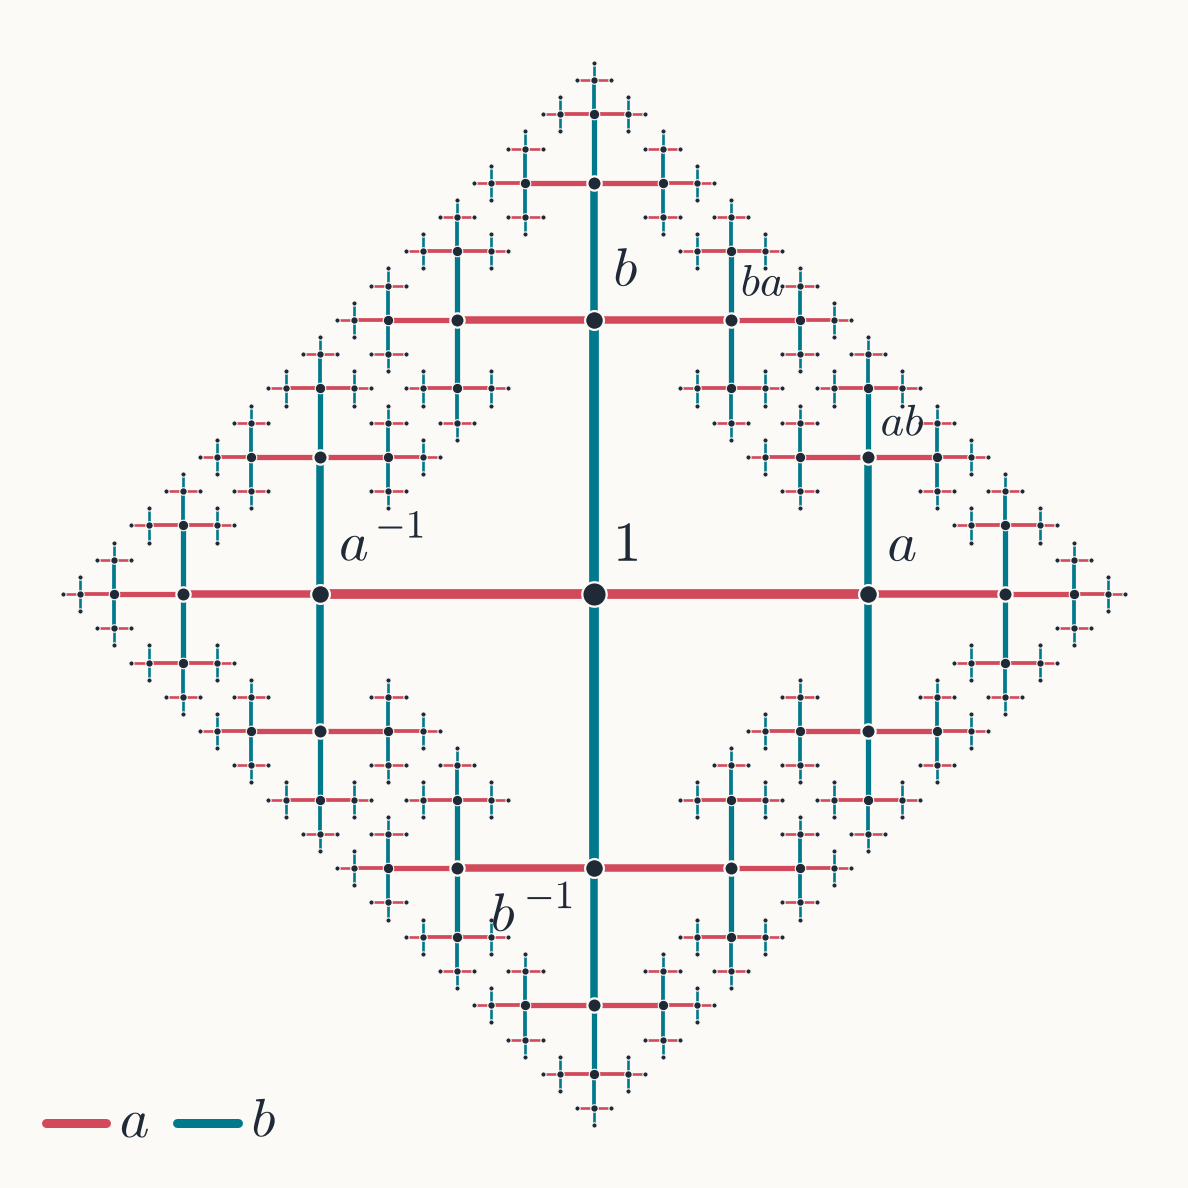
\includegraphics[width=0.40\linewidth]{cayley-tree.png}
  \caption{The Cayley graph of $F(a,b)$ out to distance $5$ from $1$:
  $2 \cdot 3^5 - 1 = 485$ vertices. Edges from $g$ to $ga$ are horizontal
  (red) and edges from $g$ to $gb$ are vertical (teal). Edge lengths halve at
  each step, so the tree fits in the plane.}
  \label{fig:tree}
\end{figure}

\subsection{The four-set form}
Here is the main statement of this project.

\begin{theorem}[Ping-pong lemma]\label{thm:pingpong}
Let a group $G$ act on a set $X$ and let $a, b \in G$. Suppose that
$D_a, D_{a^{-1}}, D_b, D_{b^{-1}} \subseteq X$ are nonempty and pairwise
disjoint, and that
\begin{equation}\label{eq:pingpong}
  s(D_t) \subseteq D_s \qquad \text{for all } s, t \in S \text{ with } t \ne s^{-1}.
\end{equation}
Then $a$ and $b$ freely generate a free group of rank~$2$.
\end{theorem}

In words: each letter $s$ maps three of the four sets, all but $D_{s^{-1}}$,
into its own set $D_s$. Figure~\ref{fig:foursets} shows the hypothesis for $a$
and for~$b$.

\begin{proof}
Let $w = s_1 s_2 \cdots s_n$ be a reduced word with $n \ge 1$. We show that
$w \ne 1$ in $G$. Since $S$ has four letters, we can choose $t \in S$ with
$t \ne s_1$ and $t \ne s_n^{-1}$. Pick $x \in D_t$.

We claim that $s_k s_{k+1} \cdots s_n x \in D_{s_k}$ for $k = n, n-1, \dots, 1$.
For $k = n$ this says $s_n x \in D_{s_n}$, which is \eqref{eq:pingpong} with
$s = s_n$, since $t \ne s_n^{-1}$. If the claim holds for $k+1$, then
$s_k s_{k+1} \cdots s_n x$ lies in $s_k(D_{s_{k+1}})$, which is contained in
$D_{s_k}$ by \eqref{eq:pingpong}, since $s_{k+1} \ne s_k^{-1}$ (the word is
reduced). This proves the claim.

For $k = 1$ the claim says $wx \in D_{s_1}$. Since $t \ne s_1$, the sets
$D_{s_1}$ and $D_t$ are disjoint, so $wx \ne x$. Hence $w$ acts nontrivially
on $X$, and $w \ne 1$ in $G$. Every element of $F(a,b)$ other than $1$ is a
nonempty reduced word, so the kernel of $\varphi$ is trivial.
\end{proof}

\begin{figure}[htbp]
  \centering
  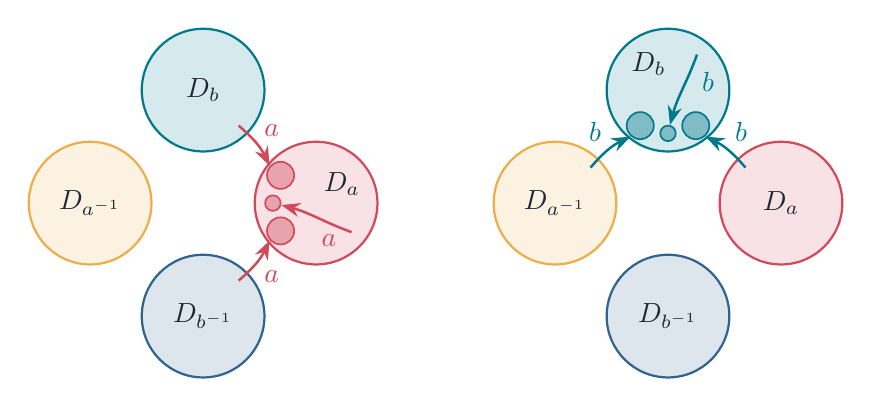
\begin{tikzpicture}[scale=0.82,
      set/.style={draw=#1, fill=#1!16, line width=0.8pt},
      img/.style={draw=#1, fill=#1!50, line width=0.6pt},
      map/.style={-{Stealth[length=2.4mm]}, line width=0.9pt, draw=#1},
      lab/.style={text=ink}]
    % Left: the letter a.
    \begin{scope}
      \draw[set=pa]  ( 1.75, 0) circle (0.95);
      \draw[set=pai] (-1.75, 0) circle (0.95);
      \draw[set=pb]  (0,  1.75) circle (0.95);
      \draw[set=pbi] (0, -1.75) circle (0.95);
      \node[lab] at (2.15, 0.3) {$D_a$};
      \node[lab] at (-1.75, 0) {$D_{a^{-1}}$};
      \node[lab] at (0, 1.75) {$D_b$};
      \node[lab] at (0, -1.75) {$D_{b^{-1}}$};
      \draw[img=pa] (1.20,  0.43) circle (0.21);
      \draw[img=pa] (1.08,  0)    circle (0.12);
      \draw[img=pa] (1.20, -0.43) circle (0.21);
      \draw[map=pa] (0.55, 1.20) to[bend left=12] node[above right=-1pt, text=pa] {$a$} (1.03, 0.58);
      \draw[map=pa] (0.55, -1.20) to[bend right=12] node[below right=-1pt, text=pa] {$a$} (1.03, -0.58);
      \draw[map=pa] (2.30, -0.45) to[out=160, in=-15] (1.21, -0.03);
      \node[text=pa] at (1.95, -0.58) {$a$};
    \end{scope}
    % Right: the letter b.
    \begin{scope}[xshift=7.2cm]
      \draw[set=pa]  ( 1.75, 0) circle (0.95);
      \draw[set=pai] (-1.75, 0) circle (0.95);
      \draw[set=pb]  (0,  1.75) circle (0.95);
      \draw[set=pbi] (0, -1.75) circle (0.95);
      \node[lab] at (1.75, 0) {$D_a$};
      \node[lab] at (-1.75, 0) {$D_{a^{-1}}$};
      \node[lab] at (-0.3, 2.15) {$D_b$};
      \node[lab] at (0, -1.75) {$D_{b^{-1}}$};
      \draw[img=pb] ( 0.43, 1.20) circle (0.21);
      \draw[img=pb] ( 0,    1.08) circle (0.12);
      \draw[img=pb] (-0.43, 1.20) circle (0.21);
      \draw[map=pb] (1.20, 0.55) to[bend right=12] node[above right=-1pt, text=pb] {$b$} (0.58, 1.03);
      \draw[map=pb] (-1.20, 0.55) to[bend left=12] node[above left=-1pt, text=pb] {$b$} (-0.58, 1.03);
      \draw[map=pb] (0.45, 2.30) to[out=-110, in=75] (0.03, 1.21);
      \node[text=pb] at (0.62, 1.88) {$b$};
    \end{scope}
  \end{tikzpicture}
  \caption{The hypothesis \eqref{eq:pingpong} for the letter $a$ (left) and
  the letter $b$ (right). The letter $a$ maps each of $D_a$, $D_b$ and
  $D_{b^{-1}}$ to one of the small dark discs inside $D_a$; nothing is
  required of $a$ on $D_{a^{-1}}$. The pictures for $a^{-1}$ and $b^{-1}$ are
  the mirror images.}
  \label{fig:foursets}
\end{figure}

\begin{remark}\label{rem:variants}
\begin{enumerate}
\item The classical \emph{Schottky hypothesis} is that
$s(X \setminus D_{s^{-1}}) \subseteq D_s$ for every $s \in S$. It implies
\eqref{eq:pingpong}, because $D_t \subseteq X \setminus D_{s^{-1}}$ whenever
$t \ne s^{-1}$. The weaker hypothesis \eqref{eq:pingpong} is the one that
Sanov's example satisfies (Remark~\ref{rem:schottky-fails}).
\item Nothing is special about two generators. For elements
$a_1, \dots, a_k$ with $k \ge 2$ and $2k$ sets $D_{a_i^{\pm1}}$, the same proof
works, since there are $2k \ge 4$ letters to choose $t$ from. For $k = 1$ the
statement is false: if $a = 1$, then $a(D_a) \subseteq D_a$ and
$a^{-1}(D_{a^{-1}}) \subseteq D_{a^{-1}}$ for any two disjoint sets.
\end{enumerate}
\end{remark}

\subsection{The two-set form}
De la Harpe~\cite{delaharpe-2000} proves a version for free products, with two
sets instead of four, and credits the idea to Klein.

\begin{theorem}[Table-tennis lemma]\label{thm:tabletennis}
Let a group $G$ act on a set $X$, and let $H_1, H_2 \le G$ be subgroups with
$\abs{H_1} \ge 3$ and $\abs{H_2} \ge 2$. Let $X_1, X_2 \subseteq X$ be nonempty
and disjoint, with
\[
  h(X_2) \subseteq X_1 \text{ for all } h \in H_1 \setminus \{1\}, \qquad
  h(X_1) \subseteq X_2 \text{ for all } h \in H_2 \setminus \{1\}.
\]
Then the natural map $H_1 * H_2 \to G$ is injective, so
$\gen{H_1, H_2} \cong H_1 * H_2$.
\end{theorem}

\begin{proof}
Every element of $H_1 * H_2$ other than $1$ is a unique alternating product
$w = h_1 h_2 \cdots h_n$ with $n \ge 1$, where each $h_i$ lies in
$H_1 \setminus \{1\}$ or in $H_2 \setminus \{1\}$ and consecutive factors lie
in different subgroups. We show that $w \ne 1$ in $G$, in four cases.

\emph{Case 1: $h_1, h_n \in H_1$.} Pick $x \in X_2$. Then $h_n x \in X_1$,
then $h_{n-1} h_n x \in X_2$, and so on, alternating. Since $h_1 \in H_1$, we
get $wx \in X_1$. As $X_1 \cap X_2 = \emptyset$, $wx \ne x$, so $w \ne 1$.

\emph{Case 2: $h_1, h_n \in H_2$.} Pick $h \in H_1 \setminus \{1\}$. Then
$h w h^{-1} = h h_1 \cdots h_n h^{-1}$ is an alternating product that begins
and ends in $H_1$, so it is not $1$ by Case~1. Hence $w \ne 1$.

\emph{Case 3: $h_1 \in H_1$ and $h_n \in H_2$.} Since $\abs{H_1} \ge 3$, we
can pick $h \in H_1$ with $h \ne 1$ and $h \ne h_1^{-1}$. Then
$h w h^{-1} = (h h_1) h_2 \cdots h_n h^{-1}$, and $h h_1 \ne 1$, so this is an
alternating product that begins and ends in $H_1$. By Case~1 it is not $1$, so
$w \ne 1$.

\emph{Case 4: $h_1 \in H_2$ and $h_n \in H_1$.} Then
$w^{-1} = h_n^{-1} \cdots h_1^{-1}$ is as in Case~3, so $w^{-1} \ne 1$ and
$w \ne 1$.
\end{proof}

\begin{remark}\label{rem:three}
The condition $\abs{H_1} \ge 3$ cannot be dropped. Let $G = \{1, \sigma\}$
act on $X = \{x_1, x_2\}$ by swapping the two points, and let
$H_1 = H_2 = G$, $X_1 = \{x_1\}$, $X_2 = \{x_2\}$. All the other hypotheses
hold, but $\gen{H_1, H_2} = G$ has order $2$, while $H_1 * H_2$ is infinite.
\end{remark}

\begin{example}\label{ex:freeproduct}
If $a$ and $b$ have infinite order, the two-set form with
$H_1 = \gen{a}$ and $H_2 = \gen{b}$ gives $\gen{a,b} \cong \Z * \Z$, a free
group of rank $2$ on $a$ and $b$. Its hypotheses concern all nonzero powers of
$a$ and $b$, but only two sets. For a free product that is not free, let
$\PSL_2(\Z)$ act on the irrational numbers by M\"obius transformations, and let
$s(x) = -1/x$ and $r(x) = 1/(1-x)$. Then $s$ has order $2$ and $r$ has
order $3$ (indeed $r^2(x) = (x-1)/x$). Let $X_1$ be the positive and $X_2$
the negative irrationals. If $x < 0$, then $r(x) \in (0,1)$ and
$r^2(x) = 1 - 1/x > 1$, so $r^{\pm1}(X_2) \subseteq X_1$, and clearly
$s(X_1) \subseteq X_2$. Theorem~\ref{thm:tabletennis} gives
$\gen{r, s} \cong \Z/3 * \Z/2$. Since $s r (x) = x - 1$, the group $\gen{r,s}$
contains $x \mapsto x + 1$ and $x \mapsto -1/x$. These two maps are well
known to generate $\PSL_2(\Z)$, so $\PSL_2(\Z) \cong \Z/3 * \Z/2$.
\end{example}

\section{Sanov's example and the family \texorpdfstring{$G_t$}{G\_t}}\label{sec:sanov}

For a real number $t$ let
\[
  A_t = \mat{1}{t}{0}{1}, \qquad B_t = \mat{1}{0}{t}{1}, \qquad
  G_t = \gen{A_t, B_t} \le \SL_2(\R).
\]
Sanov's matrices are $A = A_2$ and $B = B_2$. The group $G_t$ acts linearly on
$\R^2$, and for every integer $n$,
\[
  A_t^n(x,y) = (x + nty,\ y), \qquad B_t^n(x,y) = (x,\ ntx + y).
\]
So $A_t$ shears horizontally and $B_t$ vertically. We play ping-pong on the
two cones
\[
  X_1 = \{(x,y) : \abs{x} > \abs{y}\}, \qquad X_2 = \{(x,y) : \abs{y} > \abs{x}\},
\]
split by the sign of $xy$ into the four sets of Table~\ref{tab:sanov}.

\begin{table}[htbp]
  \centering
  \caption{Sanov's four sets. The last column states them as linear
  inequalities, without absolute values or products.}
  \label{tab:sanov}
  \begin{tabular}{@{}lll@{}}
    \toprule
    Set & Definition & As linear inequalities \\
    \midrule
    $D_A$      & $\abs{x} > \abs{y}$, $xy > 0$ & $x > y > 0$ or $x < y < 0$ \\
    $D_{A^{-1}}$ & $\abs{x} > \abs{y}$, $xy < 0$ & $x > -y > 0$ or $x < -y < 0$ \\
    $D_B$      & $\abs{y} > \abs{x}$, $xy > 0$ & $y > x > 0$ or $y < x < 0$ \\
    $D_{B^{-1}}$ & $\abs{y} > \abs{x}$, $xy < 0$ & $y > -x > 0$ or $y < -x < 0$ \\
    \bottomrule
  \end{tabular}
\end{table}

The case $t = 2$ of the next theorem is Sanov's~\cite{sanov-1947}, and the
general case is usually credited to Brenner~\cite{brenner-1955}. The proof is
the now-standard ping-pong argument; we have not compared it with the original
papers.

\begin{theorem}\label{thm:sanov}
If $t \in \R$ and $\abs{t} \ge 2$, then $A_t$ and $B_t$ freely generate a free
group of rank~$2$. In particular, Sanov's matrices $A$ and $B$ do.
\end{theorem}

\begin{proof}
Let $J = \mat{1}{0}{0}{-1}$. Then $J A_t J^{-1} = A_{-t}$ and
$J B_t J^{-1} = B_{-t}$, so replacing $t$ by $-t$ does not change the
question, and we may assume $t \ge 2$. We check the hypothesis
\eqref{eq:pingpong} of Theorem~\ref{thm:pingpong} for the sets of
Table~\ref{tab:sanov}, which are nonempty and pairwise disjoint.

Let $\varepsilon = \pm 1$. We show that $A_t^{\varepsilon}$ maps each of
$D_B$, $D_{B^{-1}}$ and $D_{A^{\varepsilon}}$ into $D_{A^{\varepsilon}}$.
Write $(x', y') = A_t^{\varepsilon}(x,y) = (x + \varepsilon t y,\ y)$.
\begin{itemize}
\item If $(x,y) \in D_B \cup D_{B^{-1}}$, then $\abs{y} > \abs{x}$, so
$t\abs{y} \ge 2\abs{y} > \abs{x}$. Hence $x'$ has the sign of
$\varepsilon t y$, and $\abs{x'} \ge t\abs{y} - \abs{x} > 2\abs{y} - \abs{y} = \abs{y}$.
So $\abs{x'} > \abs{y'}$, and $x'y' = x'y$ has the sign of
$\varepsilon t y^2$, which is the sign of $\varepsilon$.
\item If $(x,y) \in D_{A^{\varepsilon}}$, then $\varepsilon xy > 0$, so
$y \ne 0$ and $x$ has the same sign as $\varepsilon t y$. Hence
$\abs{x'} = \abs{x} + t\abs{y} > \abs{y}$, and
$x'y' = xy + \varepsilon t y^2$ has the sign of $\varepsilon$.
\end{itemize}
In both cases $(x', y') \in D_{A^{\varepsilon}}$. For $B_t$, let
$\sigma(x,y) = (y,x)$. Then $\sigma A_t \sigma = B_t$, and $\sigma$ carries
$D_{A^{\pm1}}$ to $D_{B^{\pm1}}$ and $D_{B^{\pm1}}$ to $D_{A^{\pm1}}$. So
$B_t^{\varepsilon}$ maps each of $D_A$, $D_{A^{-1}}$ and $D_{B^{\varepsilon}}$
into $D_{B^{\varepsilon}}$. Theorem~\ref{thm:pingpong} applies.
\end{proof}

\begin{figure}[htbp]
  \centering
  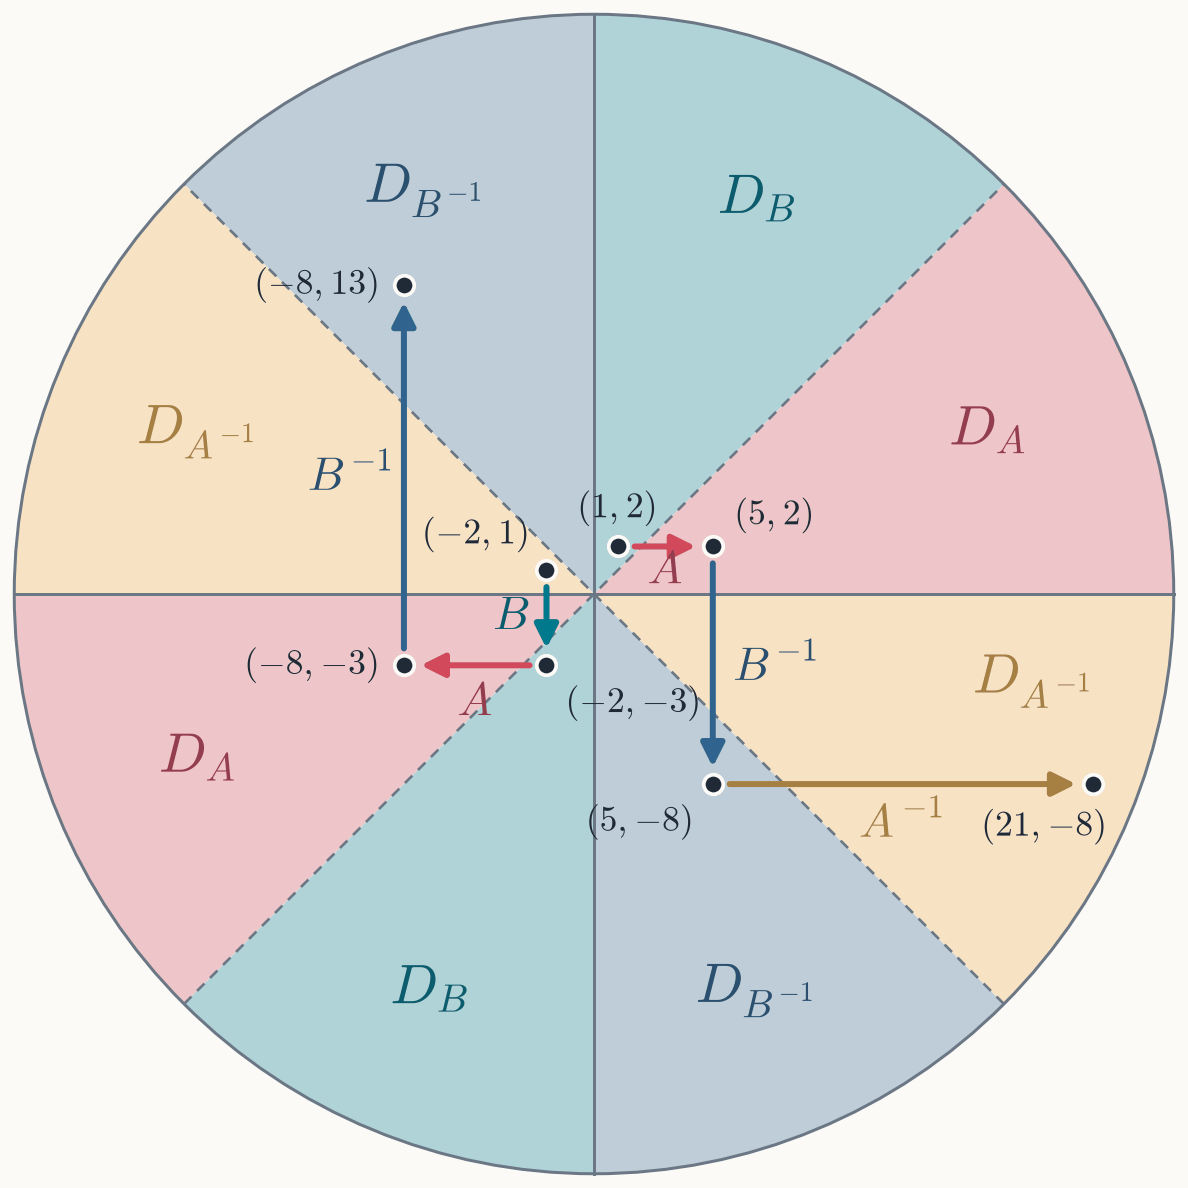
\includegraphics[width=0.48\linewidth]{cones.png}
  \caption{Sanov's sets for $t = 2$, and two short orbits starting at $(1,2)$
  and $(-2,1)$. Each arrow applies one letter, and the point lands in the set
  of that letter, as in the proof of Theorem~\ref{thm:pingpong}. The axes and
  the diagonals lie in none of the four sets.}
  \label{fig:cones}
\end{figure}

Figure~\ref{fig:cones} shows the sets for $t = 2$. The orbit of $(1,2)$, for
example, reads
\[
  (1,2) \xrightarrow{\;A\;} (5,2) \xrightarrow{\;B^{-1}\;} (5,-8)
  \xrightarrow{\;A^{-1}\;} (21,-8),
\]
so the word $A^{-1}B^{-1}A$ moves $(1,2) \in D_B$ into $D_{A^{-1}}$.

\begin{remark}\label{rem:two-cones}
Sanov's argument is often stated with the two cones and
Theorem~\ref{thm:tabletennis}. If $n \ne 0$ and $(x,y) \in X_2$, then
$\abs{x + nty} \ge \abs{n}\abs{t}\abs{y} - \abs{x} > 2\abs{y} - \abs{y} = \abs{y}$,
so $A_t^n(X_2) \subseteq X_1$. Likewise $B_t^n(X_1) \subseteq X_2$. Since
$A_t$ and $B_t$ have infinite order, Example~\ref{ex:freeproduct} gives
$G_t \cong \Z * \Z$.
\end{remark}

\begin{remark}\label{rem:schottky-fails}
The Schottky hypothesis of Remark~\ref{rem:variants} fails here: $A$ fixes
$(1,0)$, which lies outside $D_{A^{-1}}$ but not in $D_A$. This is why we use
the weaker hypothesis \eqref{eq:pingpong}. Since the sets are cones, the
argument also runs on the projective line $\RP^1$. In terms of the slope
$m = y/x$, the four sets become the intervals
\[
  D_A = (0,1), \quad D_{A^{-1}} = (-1,0), \quad D_B = (1,\infty), \quad
  D_{B^{-1}} = (-\infty,-1).
\]
Their closures touch at the slopes $0$, $\pm1$ and $\infty$. On slopes, $A$
acts by $m \mapsto m/(1+2m)$, a parabolic map whose only fixed point is the
point $0$ where $D_A$ and $D_{A^{-1}}$ meet. So the picture is like that of a
Schottky group (Section~\ref{sec:schottky}), except that the intervals touch
and the generators are parabolic.
\end{remark}

\subsection{The non-example \texorpdfstring{$t = 1$}{t = 1}}
At $t = 1$ the argument must fail, because $G_1$ is not free:
\[
  A_1 B_1^{-1} A_1 = \mat{1}{1}{0}{1} \mat{1}{0}{-1}{1} \mat{1}{1}{0}{1}
  = \mat{0}{1}{-1}{0}
\]
has order $4$. So the nonempty reduced word
\[
  (a b^{-1} a)^4 = a b^{-1} a^2 b^{-1} a^2 b^{-1} a^2 b^{-1} a
\]
is equal to $1$ in $G_1$ when $a = A_1$ and $b = B_1$. In fact $G_1 = \SL_2(\Z)$, by the classical fact that these two
elementary matrices generate $\SL_2(\Z)$. The cones fail, as they must:
$A_1(-1,2) = (1,2)$, so $A_1$ does not map $X_2$ into $X_1$. The same happens
for every $t$ with $0 < \abs{t} < 2$, since $A_t(-t/2, 1) = (t/2, 1)$ stays in
$X_2$. For such $t$ the cones say nothing, and other methods are needed;
Section~\ref{sec:open} describes what is known when $t^2$ is rational.

\section{Schottky groups}\label{sec:schottky}

A M\"obius transformation $z \mapsto (\alpha z + \beta)/(\gamma z + \delta)$,
with $\alpha\delta - \beta\gamma \ne 0$, is a bijection of the Riemann sphere
$\widehat{\C} = \C \cup \{\infty\}$ that takes circles and lines to circles
and lines. Let $D_a$, $D_{a^{-1}}$, $D_b$, $D_{b^{-1}}$ be open round discs in
$\C$ whose closures are pairwise disjoint.

Given a target disc $D$ (center $c$, radius $r$), a source disc $D'$ (center
$c'$, radius $r'$) and a complex number $u$ with $\abs{u} = 1$, consider
\begin{equation}\label{eq:pairing}
  z \longmapsto c + \frac{u\, r\, r'}{z - c'}.
\end{equation}
It sends $\infty$ to $c$ and $c'$ to $\infty$, and for other $z$ the image
lies in $D$ exactly when $\abs{z - c'} > r'$, and on $\partial D$ exactly
when $\abs{z - c'} = r'$. So it maps the circle $\partial D'$ onto
$\partial D$, and the outside $\widehat{\C} \setminus \overline{D'}$ onto
$D$. Let $a$ be such a map with $D = D_a$ and $D' = D_{a^{-1}}$, and let $b$
be one with $D = D_b$ and $D' = D_{b^{-1}}$.

As a bijection of $\widehat{\C}$, $a$ then takes the inside $D_{a^{-1}}$
onto the outside of $D_a$, so $a^{-1}$ maps
$\widehat{\C} \setminus \overline{D_a}$ onto $D_{a^{-1}}$. The same holds
for $b$. Altogether,
\[
  s\bigl(\widehat{\C} \setminus \overline{D_{s^{-1}}}\bigr) = D_s
  \qquad \text{for every } s \in S.
\]
If $t \ne s^{-1}$, then $D_t$ lies outside $\overline{D_{s^{-1}}}$, because the
closures are disjoint, so $s(D_t) \subseteq D_s$. This is the Schottky
hypothesis of Remark~\ref{rem:variants}, and Theorem~\ref{thm:pingpong} shows:

\begin{proposition}\label{prop:schottky}
The maps $a$ and $b$ freely generate a free group of rank~$2$.
\end{proposition}

A group built this way is a \emph{Schottky group} of rank~$2$.
Figure~\ref{fig:schottky} shows one, computed from the formulas.

\begin{figure}[htbp]
  \centering
  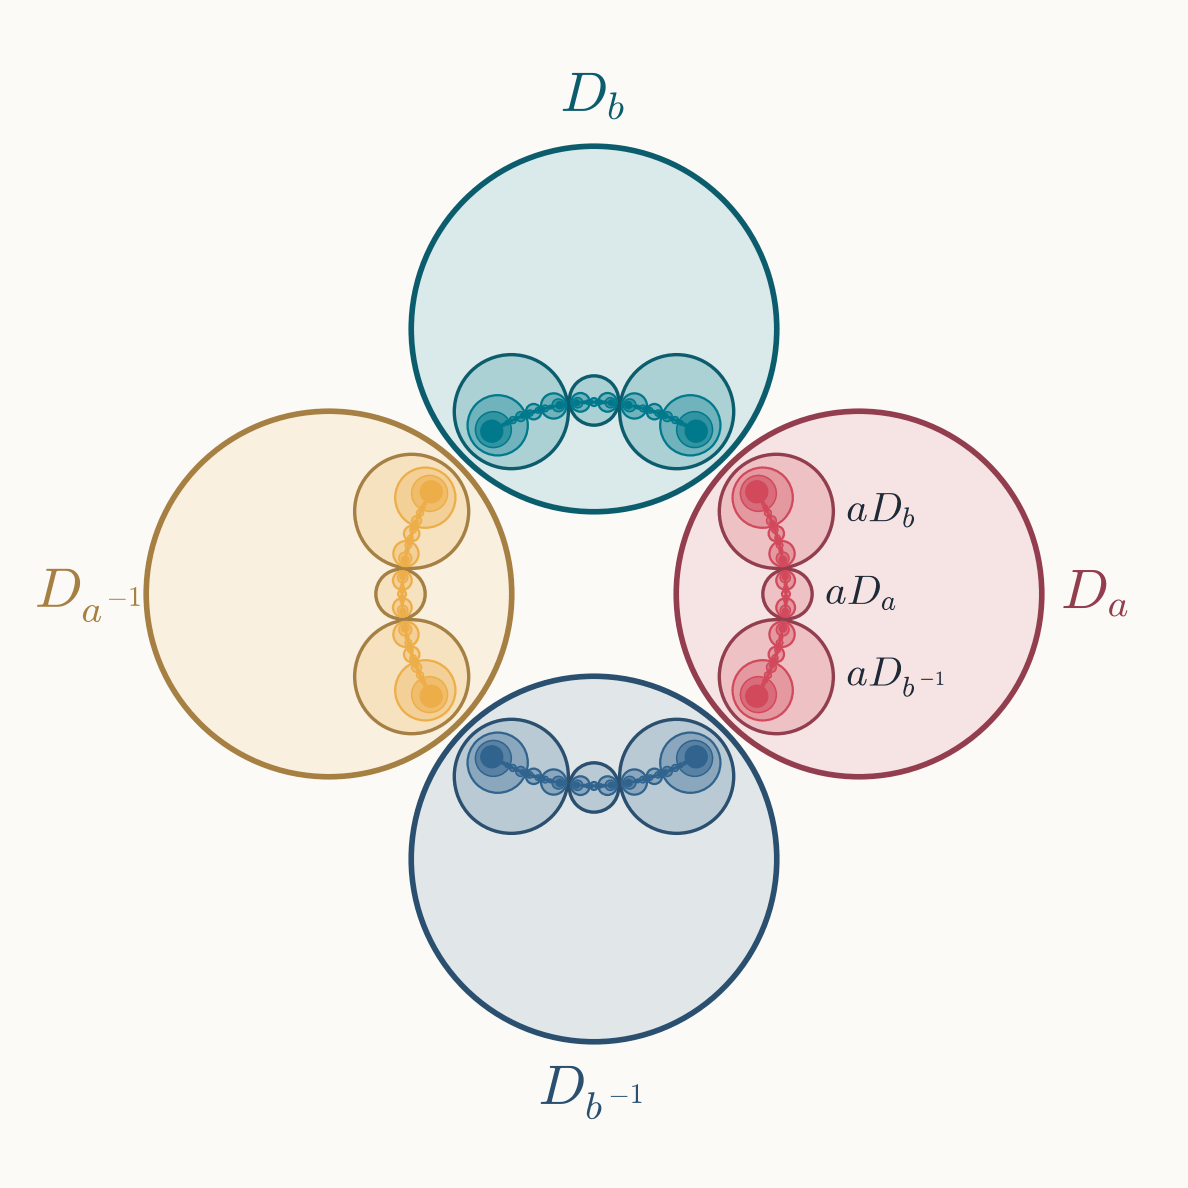
\includegraphics[width=0.48\linewidth]{schottky.png}
  \caption{A Schottky group. The discs have radius $1$ and centers $\pm 1.45$
  and $\pm 1.45i$, and \eqref{eq:pairing} gives
  $a(z) = 1.45 - 1/(z + 1.45)$ and $b(z) = 1.45i + 1/(z + 1.45i)$. Inside
  each $D_s$ are the discs $w(D_t)$ for the reduced words $wt$ of length $2$
  to $5$ that begin with $s$, darker for longer words. Here $aD_t$ means
  $a(D_t)$.}
  \label{fig:schottky}
\end{figure}

The picture is the proof of Theorem~\ref{thm:pingpong} drawn for all words
at once. If
$w = s_1 \cdots s_n$ is reduced and $t \ne s_n^{-1}$, then $w(D_t)$ is a disc
inside $D_{s_1}$. If moreover $t' \ne t^{-1}$, then
$wt(D_{t'}) \subseteq w(D_t)$, because $t(D_{t'}) \subseteq D_t$. So the discs
$w(D_t)$, one for each nonempty reduced word $wt$, are nested exactly as the
branches of the tree in Figure~\ref{fig:tree}. Call the discs with
$\abs{wt} = n$ the discs of level $n$. Discs of the same level are pairwise
disjoint, by induction on $n$, since each map is injective.

The intersection over $n$ of the unions of the closed discs of level $n$ is
the \emph{limit set} of $\gen{a,b}$. One can show that it is a Cantor set,
whose points correspond to the infinite reduced words. The closed region $F$
outside the four discs is a fundamental domain for the action on the
complement of the limit set. Gluing $\partial D_{a^{-1}}$ to $\partial D_a$
by $a$, and $\partial D_{b^{-1}}$ to $\partial D_b$ by $b$, turns $F$ into a
closed surface of genus~$2$.

\section{Ping-pong and the Tits alternative}\label{sec:tits}

\begin{theorem}[Tits~\cite{tits-1972}]\label{thm:tits}
Let $K$ be a field and let $\Gamma \le \GL_n(K)$ be a finitely generated
subgroup. Then either $\Gamma$ contains a free subgroup of rank~$2$, or
$\Gamma$ has a solvable subgroup of finite index.
\end{theorem}

The two cases exclude each other: a subgroup of a virtually solvable group is
virtually solvable, and a free group of rank~$2$ is not. The free subgroup in
Tits' proof comes from ping-pong between high powers of two well-chosen
elements. Here is the simplest instance, with a complete proof.

\begin{proposition}\label{prop:hyperbolic}
Let $g, h \in \SL_2(\R)$ with $\abs{\tr(g)} > 2$ and $\abs{\tr(h)} > 2$, and
suppose that $g$ and $h$ have no common fixed point in $\RP^1$. Then there is
$N \ge 1$ such that $g^N$ and $h^N$ freely generate a free group of rank~$2$.
\end{proposition}

\begin{proof}
Since $\abs{\tr(g)} > 2$, the matrix $g$ has real eigenvalues $\lambda$ and
$\lambda^{-1}$ with $\abs{\lambda} > 1$. Their eigenlines are the two fixed
points of $g$ in $\RP^1$: the attracting point $g^+$ (for $\lambda$) and the
repelling point $g^-$ (for $\lambda^{-1}$).

\emph{Claim.} For all open sets $U^+ \ni g^+$ and $U^- \ni g^-$ there is $N_0$
such that, for every $n \ge N_0$,
\[
  g^n(\RP^1 \setminus U^-) \subseteq U^+ \quad\text{and}\quad
  g^{-n}(\RP^1 \setminus U^+) \subseteq U^-.
\]
In a basis of eigenvectors $g = \mathrm{diag}(\lambda, \lambda^{-1})$. Give
the line through $(x,y)$ the coordinate $z = x/y \in \R \cup \{\infty\}$, so
that $g^+ = \infty$, $g^- = 0$, and $g^n$ acts by $z \mapsto \lambda^{2n} z$.
The compact set $\RP^1 \setminus U^-$ avoids $0$, so $\abs{z} \ge \delta$ on
it for some $\delta > 0$, and $U^+$ contains $\{\abs{z} > R\}$ for some $R$.
Once $\lambda^{2n}\delta > R$, the first inclusion holds. The second is the
same argument for $g^{-1}$, whose attracting point is $g^-$.

The four points $g^\pm, h^\pm$ are distinct, so they have pairwise disjoint
open neighborhoods $U_g^\pm$ and $U_h^\pm$. Choose $N$ so that the claim
holds for $g$ and for $h$ with these neighborhoods, and set $a = g^N$,
$b = h^N$ and
\[
  D_a = U_g^+, \quad D_{a^{-1}} = U_g^-, \quad D_b = U_h^+, \quad D_{b^{-1}} = U_h^-.
\]
If $t \ne a^{-1}$, then $D_t \subseteq \RP^1 \setminus U_g^-$, so
$a(D_t) \subseteq D_a$. The other three letters work the same way, and
Theorem~\ref{thm:pingpong} applies.
\end{proof}

\begin{proof}[Sketch of the general case]
This is an outline, not a proof; the details are the heart
of~\cite{tits-1972}. Let $k$ be a local field, such as $\R$, $\C$ or the
$p$-adic numbers $\Q_p$. Call $g \in \GL_n(k)$ \emph{proximal} if it has a
unique eigenvalue of largest absolute value, and that eigenvalue is simple.
On the projective space $\mathbb{P}(k^n)$, high powers of $g$ push everything
that stays away from a repelling hyperplane (the sum of the other generalized
eigenspaces) close to an attracting point (the eigenline of that
eigenvalue). Hyperbolic elements of $\SL_2(\R)$ are the case $n = 2$.
\begin{enumerate}
\item \emph{Ping-pong.} If $g^{\pm1}$ and $h^{\pm1}$ are all proximal, and each
attracting point lies off the repelling hyperplanes of the other element and
its inverse, then the proof of Proposition~\ref{prop:hyperbolic}, with small
neighborhoods of the four attracting points as the sets $D_s$, shows that
$g^N$ and $h^N$ freely generate a free group of rank~$2$ for large $N$.
\item \emph{Finding such elements.} If $\Gamma$ is not virtually solvable, one
reduces to the case where its Zariski closure is semisimple. One then embeds
the field generated by the matrix entries of $\Gamma$ into a local field $k$,
chosen so that some $\gamma \in \Gamma$ has eigenvalues of different absolute
values. A suitable representation, such as an exterior power, makes $\gamma$
proximal, and Zariski density supplies a conjugate of $\gamma$ in general
position with respect to $\gamma$. \qedhere
\end{enumerate}
\end{proof}

The choice of local field matters: a compact group such as $\SO_3(\R)$ acts
on the real projective plane by isometries, so the contraction has to be found
over another local field, for example a $p$-adic one. Breuillard and Gelander~\cite{breuillard-gelander-2007} proved a
topological version of the alternative, in which ping-pong on projective
spaces over local fields produces free subgroups that are dense, for example
in compact Lie groups.

\section{An open question}\label{sec:open}

Ping-pong proves that a group is free. It cannot prove that a group is not
free; for that one needs a relation. This section describes a family where
the two kinds of argument meet, in the normalization of Kim and
Koberda~\cite{kim-koberda-2019}. For $q \in \R$ let
\[
  a = \mat{1}{0}{1}{1}, \qquad b_q = \mat{1}{q}{0}{1}, \qquad
  G_q = \gen{a, b_q}.
\]
For $t \ne 0$, conjugating by $\mathrm{diag}(t, 1)$ carries $A_t$ to $b_{t^2}$
and $B_t$ to $a$. So $G_t$ of Section~\ref{sec:sanov} is conjugate to $G_q$
with $q = t^2$: Sanov's group is $q = 4$ and $\SL_2(\Z)$ is $q = 1$.
Conjugating by $\mathrm{diag}(1,-1)$ carries $a$ to $a^{-1}$ and $b_q$ to
$b_{-q}$, so $G_q$ and $G_{-q}$ are conjugate.

\begin{proposition}\label{prop:q-free}
If $\abs{q} \ge 4$, then $a$ and $b_q$ freely generate a free group of
rank~$2$.
\end{proposition}

\begin{proof}
Let $U = \{(x,y) : \abs{x} > 2\abs{y}\}$ and
$V = \{(x,y) : \abs{x} < 2\abs{y}\}$, and let $n \ne 0$. If $(x,y) \in U$,
then $a^n(x,y) = (x,\ nx + y)$ and
$\abs{nx + y} \ge \abs{x} - \abs{y} > \abs{x} - \abs{x}/2 = \abs{x}/2$, so
$a^n(U) \subseteq V$. If $(x,y) \in V$, then $b_q^n(x,y) = (x + nqy,\ y)$
and $\abs{x + nqy} \ge 4\abs{y} - \abs{x} > 2\abs{y}$, so
$b_q^n(V) \subseteq U$. Both $a$ and $b_q$ have infinite order, so
Theorem~\ref{thm:tabletennis} with $H_1 = \gen{b_q}$, $X_1 = U$,
$H_2 = \gen{a}$, $X_2 = V$ gives $G_q \cong \Z * \Z$.
\end{proof}

For $\abs{q} < 4$ these sets fail. The question is what happens there for
rational~$q$.

\begin{question}\label{q:rational}
Is $G_q$ non-free for every nonzero rational $q$ with $\abs{q} < 4$?
\end{question}

(At $q = 0$, $b_0 = 1$ and $G_0 = \gen{a} \cong \Z$, which is free of rank~$1$.) For $q = 1, 2, 3$ a single element
gives a relation: $a b_q^{-1} = \mat{1}{-q}{1}{1-q}$ has trace $2 - q$, which
is $1$, $0$ or $-1$. A matrix in $\SL_2$ with one of these traces has
eigenvalues that are primitive roots of unity of order $6$, $4$ or $3$, and
the two eigenvalues are distinct, so it has that finite order. Hence
$(a b_q^{-1})^{12} = 1$, a relation given by a nonempty reduced word, and
$G_q$ is not free. By the symmetry $q \mapsto -q$ the same holds for
$q = -1, -2, -3$.

For other rational $q$ in $(-4,4)$ the question is harder. Kim and
Koberda~\cite{kim-koberda-2019} prove (arXiv:1901.06375) that $G_q$ is not
free when $q = s/r$ with $\abs{s} \le 27$, except possibly when $s = 24$; for
$s = 24$ they show that the denominators $r$ giving a non-free group have
natural density~$1$. Some of their proofs are computer assisted.
Nyberg-Brodda~\cite{nyberg-brodda-2023} (arXiv:2312.11258) conjectures that
when $q = m/p$ in this range, with $p$ prime, $G_q$ is an explicit congruence
subgroup of $\SL_2(\Z[\frac1p])$, and proves this when $m \le 4$ and in some cases with
$m = 5$. In those cases $G_q$ has finite index in $\SL_2(\Z[\frac1p])$, so it
is far from free. Questions of this kind go back to the study by Lyndon and
Ullman~\cite{lyndon-ullman-1969} of which complex parameters make two
parabolic transformations generate a free group.

\section{In this project}\label{sec:project}

This paper is part of an AlphaCentaur demo project, whose other files tell
the same story in other forms. They are pointers only: the paper does not
depend on them or make claims about what they currently check or print; their
own sections in AlphaCentaur show that.

\begin{itemize}
\item \emph{Formalization.} The four-set lemma, Theorem~\ref{thm:pingpong},
is formalized in Lean in the file \projectfile{lean/PingPong/Lemma.lean}, which
uses the reduced words of \projectfile{lean/PingPong/Words.lean}. Sanov's case,
Theorem~\ref{thm:sanov} with $t = 2$, is formalized in
\projectfile{lean/PingPong/Sanov.lean}. There the matrices act on $\Z^2$ and
the four sets are given by the linear inequalities of Table~\ref{tab:sanov},
so each inclusion is a statement of linear integer arithmetic. The
Formalization section records whether these files check.
\item \emph{Computations.} The alphaPy notebook
\projectfile{computations/ping_pong.py} checks Sanov's case by computer, with
exact arithmetic: it multiplies out reduced words in $A$ and $B$. It also
searches for relations in the groups $G_q$ of Section~\ref{sec:open}. Its
recorded runs are in the Computations section.
\item \emph{Pictures and talk.} The app
\projectfile{apps/ping-pong-explorer} draws Schottky discs and Sanov's cones
interactively, and the slides in \projectfile{talks/ping-pong} present the
lemma as a talk.
\end{itemize}


\bibliographystyle{amsplain}
\bibliography{alphacentaur}

\end{document}
